% !TEX root = MutationTestingSurvey.tex

\subsection{Solutions to Improve Compile-time Scalability}
\label{sub:compileTime}
\label{sec:opt:selection}

Another source of \INDEX{scalability issues} is the compilation of mutants;
indeed, because of the large number of mutation operators available in the literature, the number of mutants to be compiled is not negligible. In this section we report the main research results aiming at reducing the time required to compile mutants.
%has worked on approaches based on optimising the compilation process.

Untch et al. \cite{untch1993mutation} proposed a technique called \INDEX{mutant schemata}; the technique introduces the concept of meta-program, which stands for including and compiling all the mutants in a single executable file, instead of compiling one executable per mutation generated. The mutations are then managed at run-time through parameters that enable software engineers to choose the mutation to be executed, results show speed improvements over 300\% \cite{untch1993mutation,papadakis2010automatic}. Modern mutation testing tools such as Accmut \cite{wang2017faster} and Milu \cite{jia2008milu} include this type of optimisation.

Another solution consists of mutating directly the compiled code so that mutants can be executed without compiling each of them.
This optimisation has been applied on 
Assembly languages \cite{crouzet2006sesame},
Java bytecode \cite{ma2006mujava}, 
binary code for embedded software \cite{becker2012xemu},
Common Intermediate Language (.NET) \cite{derezinska2011object} 
and LLVM Intermediate Representation \cite{hariri2016evaluating}. 
% \REVTWO{C8}{Results obtained by Derezinska and Kowalski \cite{derezinska2011object} show that, on average, the mutation testing process mutating compiled code requires only 50\% of the time required by a traditional mutation testing process applied to source code. 
% Additionally, the mutations performed on compiled code can be applied directly to multiple source languages (e.g., LLVM IR supports C, C++, Objective-C, Objective-C++, OpenMP, OpenCL and CUDA) \cite{hariri2019comparing}.
% However, there are some drawbacks when mutating compiled code, for example many of the mutations generated cannot be represented at the source code level \cite{jia2010analysis}, creating not relevant mutations. 
% In the case of mutation of binary code, the mutation process can become very expensive since it is necessary to translate the code into machine readable instructions \cite{becker2012xemu}.}



%\DONE{I think we need here a paragraph where you say that LLVM IR is a common target of multiple research work. You can reuse the text in A1.3.1 CLANG/LLVM, along with the picture.}

Among the available solutions for the analysis of compiled code, the LLVM project, whose process is shown in Figure~\ref{fig:compileTime:llvm}, is the mostly adopted by researchers in recent years. It consists of a set of compiler and toolchain technologies. LLVM is designed around an intermediate representation (i.e., LLVM IR) that serves as a portable, high-level assembly language useful for code optimizations. LLVM was originally implemented for the C and C++ programming langauges, but currently it also supports Ada, D, Delphi, Fortran, Haskell, Julia, Objective-C, Rust and Swift. It can be used for performing static analysis on code (e.g., uninitialized memory uses), optimization, or code parsing.
LLVM IR is a common target of multiple research work, and many mutation toolsets rely on it (e.g., Mull~\cite{denisov2018mull}, SRCIRor~\cite{hariri2018srciror,hariri2019comparing} and Accmut~\cite{wang2017faster}).

	\begin{figure}
	\centering
		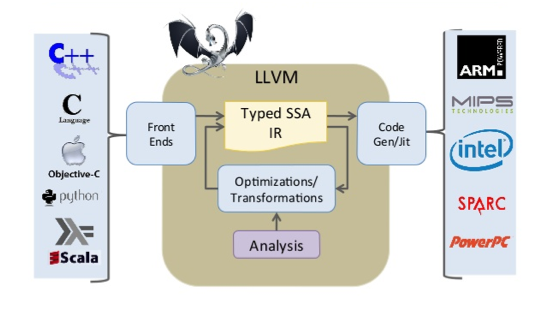
\includegraphics[width=0.7\textwidth]{images/llvm}
		\caption{LLVM compiler infrastructure.}
		\label{fig:compileTime:llvm}
	\end{figure}

%Clang is a front-end for LLVM that processes C-family languages: C, C++, Objective C, Objective C++. Clang converts C/C++ to LLVM IR, LLVM performs optimizations on the IR, and the LLVM x86 backend writes out x86 machine code for execution.



%\DONE{In the paragraph below it is not clear what do you mean for 'compiled code', I expect a follow-up sentence where you specify the type of compiled code they consider in their experiments.} 

%\DONE{In general, If the experiments below target LLVM IR say it explicitly}

\REVTWO{C8}{About the advantages of performing mutation at different levels,
the results obtained by Derezinska and Kowalski~\cite{derezinska2011object} show that, on average, the mutation of compiled code requires only 50\% of the time required by a traditional mutation testing process applied to source code. The type of compiled code they consider in their experiments was the Common Intermediate Language (.NET).}
%\DONE{The following sentence is unclear. Do you mean that toolsets that work on IR can be easily adopted to work on multiple languages?}
\REVTWO{C8}{Additionally, the mutation toolsets that work on IR can be easily adopted to work on multiple source languages,
%performed on compiled code can be applied directly to multiple source languages, 
for example, LLVM IR supports C, C++, Objective-C, Objective-C++, OpenMP, OpenCL and CUDA~\cite{hariri2019comparing}.}

%\DONE{Can you report some numbers? is it binary code or executable code or executable binary code (i.e., .EXE programs)?}
Advantages had been also acknowledge on the mutation of binaries. Becker et al.~\cite{becker2012xemu}, empirically observed that the overall time of the mutation process can be 
substantially reduced (up to 50\%) when mutation operators are applied to ARM binaries instead of source code.

The mutation of IR code also facilitates the integration of optimizations that require dynamic program analysis (i.e., the analysis of data collected at runtime~\cite{Pezze:Book}). An example is given by the optimizations implemented by Mull~\cite{denisov2018mull}, an open source tool for mutation testing of C/C++ software based on the LLVM framework. By leveraging LLVM IR, Mull generates mutants on the fly, while the SUT is executed against the test suite. To this end it relies on the JIT feature of LLVM. This feature enables the compilation of code on the fly as it is needed, with no necessity of re-compiling the whole program on disk. The online nature of Mull enables it to implement a set of optimizations that speed up the mutation process. A list of optimizations follows:
\begin{itemize}
	\item Dynamic Call Tree: optimization for mutating source code reachable by the test cases.
	\item LLVM JIT engine: compilation and linking of the new mutants happen in memory, thus there is no disk I/O overhead.
	\item Sandboxing: run each test in a separate child process, this way, if the child process fails it will not affect the parent process.
	\item Dry-run: collect information in advance about how many mutations a project has and how much time does it take to run it.
	\item Caching: save mutants on disk; for future executions Mull tries first loading the object file from the cache first.
	\item Fail-fast mode: once a mutant is killed by a test case it is no longer executed against other test cases.
\end{itemize}


%On a different context, such as the mutation of ARM binaries, the mutation process can become very expensive since it is necessary to translate the code into machine readable instructions before performing actual mutations~\cite{becker2012xemu}.

%\DONE{Below, an example is needed. Also add a sentence that indicates which type of compiled code was considered Can you present the solutions invented by MULL to overcome this problem? Can you present the features of MULL in a dedicated paragraph?}


\REVTWO{C8}{Unfortunately, the mutation of compiled code is not exempt from \EMPH{drawbacks}. For example, an empirical evaluation performed by Schuler et al.~\cite{schuler2009efficient} shows that many mutants generated on Java bytecode cannot be represented at the source code level, which indicates that they are not representative of real faults.
This problem has been observed also in other programming languages such as C++. For instance, the LLVM IR compilation of the C++ standard library method \texttt{std::vector::push\_back} produces near 200 LLVM IR instructions, all of which might be mutated, even if they lead to the generation of compiled code that it is impossible to be generated by modifying the source code (these are called \INDEX{junk mutants} in Mull~\cite{denisov2018mull}). 
For this reason, Mull checks for each mutation generated at LLVM IR level its representation on the source code, in the case a mutation cannot be represented then is discarded.
To minimize the consequences of this problem, for every mutant, Mull implements a heuristic filter that retrieves the AST node that has been targeted by the mutation and identifies a junk mutant based on the information associated to the AST node. For example, nodes without associated source code or nodes whose source file is a system library headers should not be mutated\footnote{Implementation details can be found in the Mull component \emph{lib/JunkDetection/CXX/CXXJunkDetector.cpp}}. Mull authors report that, for C and C++ projects, this approach eliminates the vast majority of junk mutations~\cite{denisov2018mull}.
%
%Mull has implemented further optimizations to overcome this limitation~\cite{denisov2018mull}.}
%
Related to this, recently Hariri et al.~\cite{hariri2019comparing} provided empirical evidence that \textit{the number of generated mutants is much higher at the intermediate representation level than at source code level, suggesting that mutation testing at source code level is much faster to perform than at intermediate representation level.}}




